\chapter{多次元配列}
\label{chap:multidimensional-arrays}

この章では、2次元配列を使って、表や盤面のようなデータを扱う方法を学びます。第10章では、配列を使って複数の円や棒の長さをまとめて扱いました。そこでは、\texttt{circleX[0]}、\texttt{circleX[1]}のように、1つの添え字番号で要素を選びました。

格子状に並んだマス、ゲームの盤面、画像のピクセルに近い情報を扱うときは、「何番目の行か」と「何番目の列か」の2つで場所を指定できると便利です。このようなデータを扱うために、2次元配列を使います。

\section{この章の概要}

この章では、色の格子、クリックされた場所の記録、オセロ風の盤面を題材に、2次元配列の使い方を学びます。

この章で扱う主な内容は次の通りです。

\begin{itemize}
    \item 2次元配列の考え方
    \item 行と列を使った要素の指定
    \item 2次元配列の型と\texttt{length}を使った行・列数
    \item 二重の\texttt{for}文
    \item マウス座標から行と列を求める方法
    \item 盤面を2次元配列で表す方法
\end{itemize}

\section{2次元配列とは何か}

2次元配列は、配列の中に配列が入っている形のデータです。1次元配列が横一列の箱だとすると、2次元配列は行と列を持つ表のようなものとして考えられます。

\begin{figure}[htbp]
    \centering
    \begin{tikzpicture}[
        cell/.style={rectangle, draw, minimum width=18mm, minimum height=10mm, align=center},
        index/.style={align=center}
    ]
        \foreach \row in {0,1,2} {
            \foreach \column in {0,1,2,3} {
                \node[cell] at (\column*1.8, -\row*1.0)
                    {\texttt{[\row][\column]}};
            }
        }
        \foreach \row in {0,1,2} {
            \node[index] at (-1.2, -\row*1.0) {行\\\texttt{\row}};
        }
        \foreach \column in {0,1,2,3} {
            \node[index] at (\column*1.8, 0.8) {列\\\texttt{\column}};
        }
    \end{tikzpicture}
    \caption{2次元配列を行と列で考える}
    \label{fig:chapter13-row-column}
\end{figure}

TypeScriptでは、数値の2次元配列を\texttt{number[][]}と書きます。これは「\texttt{number[]}の配列」、つまり「数値の配列が並んだもの」と読むこともできます。

\begin{pointbox}{添え字は2つになる}
2次元配列では、\texttt{numbers[row][column]}のように添え字を2つ使います。この章では、1つ目を行、2つ目を列として読むことにします。
\end{pointbox}

\section{表のように数値を表示する}

まずは、数値を2次元配列に保存し、表のように表示するプログラムを見てみます。行と列を使って、どのマスにどの値を表示するかを決めます。

\begin{listing}[htbp]
\inputminted{ts}{listings/chapter13/grid-numbers.ts}
\caption{2次元配列の数値を表のように表示する}
\label{lst:chapter13-grid-numbers}
\end{listing}

\texttt{numbers[0][0]}は左上の値、\texttt{numbers[0][1]}は同じ行の次の値を表します。\texttt{numbers[1][0]}は、1行下がった最初の値です。

\begin{center}
\begin{tabular}{lll}
\toprule
式 & 表す場所 & 値 \\
\midrule
\texttt{numbers[0][0]} & 0行0列 & \texttt{1} \\
\texttt{numbers[0][3]} & 0行3列 & \texttt{4} \\
\texttt{numbers[2][0]} & 2行0列 & \texttt{9} \\
\texttt{numbers[2][3]} & 2行3列 & \texttt{12} \\
\bottomrule
\end{tabular}
\end{center}

\begin{notebox}{行と列の順番を決めて読む}
本書では、2次元配列の添え字を\texttt{[row][column]}の順に統一します。
\end{notebox}

\section{二重のfor文}

2次元配列のすべての要素を調べるには、\texttt{for}文を2つ重ねます。外側の\texttt{for}文で行を選び、内側の\texttt{for}文でその行の列を順番に選びます。

\begin{figure}[htbp]
    \centering
    \begin{tikzpicture}[
        cell/.style={rectangle, draw, minimum width=16mm, minimum height=9mm, align=center},
        arrow/.style={->, thick}
    ]
        \foreach \row in {0,1,2} {
            \foreach \column in {0,1,2,3} {
                \node[cell] (c\row\column) at (\column*1.6, -\row*0.9)
                    {\texttt{\row,\column}};
            }
        }
        \draw[arrow, red] (c00.north) to[bend left=20] (c01.north);
        \draw[arrow, red] (c01.north) to[bend left=20] (c02.north);
        \draw[arrow, red] (c02.north) to[bend left=20] (c03.north);
        \draw[arrow, blue] (c03.east) to[bend left=20] (c10.east);
        \draw[arrow, red] (c10.north) to[bend left=20] (c11.north);
        \draw[arrow, red] (c11.north) to[bend left=20] (c12.north);
        \draw[arrow, red] (c12.north) to[bend left=20] (c13.north);
        \node[align=left] at (3.2, -3.3)
            {赤: 列を進める\\青: 次の行へ進む};
    \end{tikzpicture}
    \caption{二重の\texttt{for}文で行と列を順に見る}
    \label{fig:chapter13-nested-loop}
\end{figure}

サンプル\ref{lst:chapter13-grid-numbers}では、\texttt{row}と\texttt{column}を使って、描画位置も計算しています。列が増えると右へ進み、行が増えると下へ進みます。

\begin{pointbox}{外側が行、内側が列}
表や盤面を左上から順に処理するときは、外側の\texttt{for}文で行、内側の\texttt{for}文で列を動かすと読みやすくなります。
\end{pointbox}

\section{\texttt{length}で行数と列数を調べる}

2次元配列では、\texttt{values.length}で行数を調べられます。ある行の列数は、\texttt{values[row].length}で調べます。これは、2次元配列が「配列の中に配列が入っている形」だからです。

\begin{listing}[htbp]
\inputminted{ts}{listings/chapter13/sum-grid.ts}
\caption{\texttt{length}を使って2次元配列の合計を求める}
\label{lst:chapter13-sum-grid}
\end{listing}

\texttt{sumGrid}関数は、\texttt{number[][]}型の引数を受け取り、すべての要素を足して返します。第8章で学んだ関数、第10章で学んだ配列、第7章で学んだ繰り返しを組み合わせた例です。

\section{色の格子を作る}

p5.jsでは色を\texttt{p5.Color}型で扱います。\texttt{p5.Color[][]}は色の2次元配列で、格子の各マスの色を保存できます。

\begin{listing}[htbp]
\inputminted{ts}{listings/chapter13/random-color-grid.ts}
\caption{\texttt{p5.Color[][]}で色の格子を作る}
\label{lst:chapter13-random-color-grid}
\end{listing}

このサンプルでは、\texttt{cellColors[row][column]}に各マスの色を保存しています。まず\texttt{cellColors[row] = [];}で1行分の配列を用意し、その後で各列の色を入れています。

\begin{notebox}{行を先に用意する}
\texttt{cellColors[row][column]}に値を入れる前に、\texttt{cellColors[row] = [];}でその行を作っておく必要があります。行を作らないまま列の値を入れようとすると、実行時にエラーになります。
\end{notebox}

\section{クリックしたマスを覚える}

2次元配列は、マスごとの状態を覚える用途にも向いています。たとえば、「そのマスが塗られているかどうか」は\texttt{boolean}型で表せます。これを格子全体に広げると\texttt{boolean[][]}になります。

\begin{listing}[htbp]
\inputminted{ts}{listings/chapter13/click-toggle-grid.ts}
\caption{\texttt{boolean[][]}でクリックしたマスを切り替える}
\label{lst:chapter13-click-toggle-grid}
\end{listing}

マウスの座標はピクセル単位です。一方、配列の添え字は0、1、2のような整数です。そのため、\texttt{Math.floor(p.mouseX / cellSize)}のようにして、マウスのx座標から列番号を求めます。

\begin{figure}[htbp]
    \centering
    \begin{tikzpicture}[
        font=\small,
        calculation/.style={draw, rounded corners=2pt, fill=blue!5, minimum width=42mm, minimum height=9mm, align=center},
        result/.style={draw, rounded corners=2pt, fill=green!8, minimum width=35mm, minimum height=9mm, align=center}
    ]
        \foreach \row in {0,1,2,3} {
            \foreach \column in {0,1,2,3,4} {
                \draw[gray] (\column*1.05,-\row*1.05)
                    rectangle +(1.05,-1.05);
            }
        }
        \fill[orange!25] (2.10,-1.05) rectangle +(1.05,-1.05);
        \draw[orange!80!black, very thick]
            (2.10,-1.05) rectangle +(1.05,-1.05);
        \fill[red!75!black] (2.36,-1.66) circle (2.2pt);

        \foreach \column in {0,1,2,3,4} {
            \node[font=\scriptsize] at (\column*1.05+0.525,0.28)
                {列\column};
        }
        \foreach \row in {0,1,2,3} {
            \node[font=\scriptsize, anchor=east]
                at (-0.12,-\row*1.05-0.525) {行\row};
        }
        \node[align=center, anchor=north] at (2.62,-4.45)
            {クリック位置\\\texttt{(135, 95)}};
        \draw[->, red!75!black, thick]
            (2.62,-4.32) -- (2.38,-1.82);

        \node[calculation] (mouse) at (9.6,0)
            {\texttt{p.mouseX = 135}、\texttt{p.mouseY = 95}};
        \node[calculation] (columnCalc) at (7.45,-1.55)
            {\texttt{135 / 60 = 2.25}\\x座標をマス幅で割る};
        \node[calculation] (rowCalc) at (11.75,-1.55)
            {\texttt{95 / 60 = 1.58...}\\y座標をマス高さで割る};
        \node[result] (columnResult) at (7.45,-3.05)
            {\texttt{Math.floor(...)}\\\texttt{column = 2}};
        \node[result] (rowResult) at (11.75,-3.05)
            {\texttt{Math.floor(...)}\\\texttt{row = 1}};
        \node[result, minimum width=56mm] (array) at (9.6,-4.55)
            {\texttt{isPainted[row][column]}\\
             \texttt{isPainted[1][2]}};

        \draw[->, thick] (mouse.south west) -- (columnCalc.north);
        \draw[->, thick] (mouse.south east) -- (rowCalc.north);
        \draw[->, thick] (columnCalc) -- (columnResult);
        \draw[->, thick] (rowCalc) -- (rowResult);
        \draw[->, thick] (columnResult.south) -- (array.north west);
        \draw[->, thick] (rowResult.south) -- (array.north east);
    \end{tikzpicture}
    \caption{マウス座標からクリックされた行と列を求める流れ}
    \label{fig:chapter13-mouse-to-row-column}
\end{figure}

図\ref{fig:chapter13-mouse-to-row-column}では、マスの大きさを60ピクセルとしています。x座標から列番号を、y座標から行番号を別々に求め、最後に\texttt{isPainted[row][column]}の順で配列の要素を選びます。

\begin{center}
\begin{tabular}{lll}
\toprule
計算 & 意味 & 例 \\
\midrule
\texttt{p.mouseX / cellSize} & x座標をマスの大きさで割る & \texttt{135 / 60 = 2.25} \\
\texttt{Math.floor(...)} & 小数点以下を切り捨てる & \texttt{2.25}から\texttt{2} \\
\texttt{isPainted[row][column]} & クリックされたマスの状態 & \texttt{true}または\texttt{false} \\
\bottomrule
\end{tabular}
\end{center}

\begin{notebox}{整数の添え字を作る}
TypeScriptの\texttt{number}型では、整数と小数を分けません。配列の添え字として使う値は、\texttt{Math.floor}で小数点以下を切り捨てて整数にしてから使います。
\end{notebox}

\begin{mistakebox}{範囲外の添え字に注意する}
マウスがキャンバスの外や端にあると、存在しない行や列を指定してしまうことがあります。サンプルでは、\texttt{0 <= row}や\texttt{row < isPainted.length}を使って、範囲内かどうかを確認してから配列を書き換えています。
\end{mistakebox}

\section{盤面を2次元配列で表す}

2次元配列は、ボードゲームの盤面を表すときにもよく使われます。ここでは、オセロのルールをすべて作るのではなく、「4行4列の小さな盤面に黒と白の石を置く」という部分だけを作ります。

\begin{listing}[htbp]
\inputminted[firstline=1,lastline=45]{ts}{listings/chapter13/simple-board.ts}
\caption{\texttt{number[][]}で簡単な盤面を表す前半}
\label{lst:chapter13-simple-board-draw}
\end{listing}

\begin{listing}[htbp]
\inputminted[firstline=47,lastline=67]{ts}{listings/chapter13/simple-board.ts}
\caption{\texttt{number[][]}で簡単な盤面を表す後半}
\label{lst:chapter13-simple-board-click}
\end{listing}

\texttt{board[row][column]}には、マスの状態を表す数値を保存しています。\texttt{empty}は何も置かれていないマス、\texttt{black}は黒い石、\texttt{white}は白い石です。サンプルは1つのファイルですが、紙面では読みやすいように前半と後半に分けて掲載しています。

\begin{figure}[htbp]
    \centering
    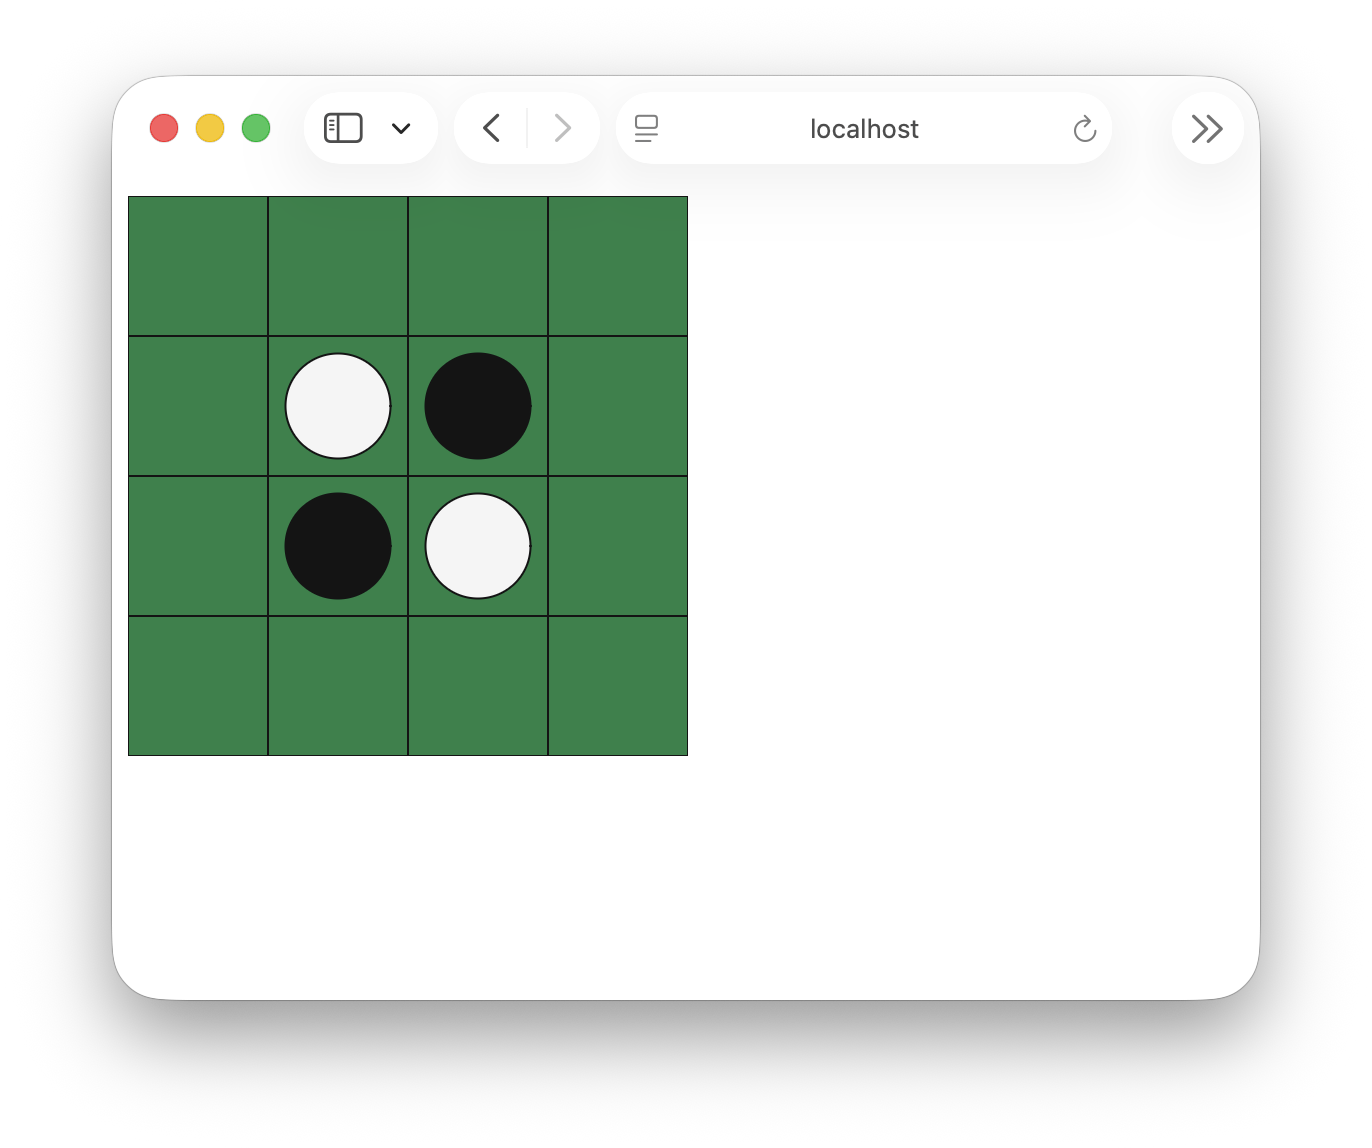
\includegraphics[
        width=0.50\linewidth,
        trim=50 174 326 35,
        clip
    ]{figures/chapter13/board.png}
    \caption{2次元配列の値から描いた4行4列の盤面}
    \label{fig:chapter13-simple-board-result}
\end{figure}

図\ref{fig:chapter13-simple-board-result}では、2次元配列の各要素が1つのマスに対応しています。\texttt{empty}のマスには石を描かず、\texttt{black}と\texttt{white}のマスにはそれぞれ黒と白の円を描いています。

\begin{pointbox}{数値に意味の名前を付ける}
\texttt{0}、\texttt{1}、\texttt{2}を直接コードの中に書くと、あとで読んだときに意味が分かりにくくなります。\texttt{empty}、\texttt{black}、\texttt{white}のような名前を付けると、盤面の状態を読みやすくできます。
\end{pointbox}

\section{よくある間違い}

2次元配列では、添え字が2つあるため、1次元配列よりも間違える場所が増えます。特に、行と列の順番、行の初期化、範囲外アクセスに注意しましょう。

\begin{mistakebox}{行と列を逆にしてしまう}
\texttt{board[row][column]}で統一しているのに、途中で\texttt{board[column][row]}と書くと、思った場所と違うマスを操作してしまいます。変数名を\texttt{row}、\texttt{column}にしておくと読み間違いを減らせます。
\end{mistakebox}

\begin{mistakebox}{行の配列を作り忘れる}
\texttt{cellColors[row][column]}に値を入れる前に、\texttt{cellColors[row] = [];}が必要です。2次元配列は、外側の配列と内側の配列を順に用意する、と考えましょう。
\end{mistakebox}

\begin{mistakebox}{すべての行の列数が同じだと思い込む}
TypeScriptの2次元配列は、行ごとに列数が違っていても作れてしまいます。そのため、列数を調べるときは\texttt{values[0].length}だけでなく、繰り返し中の\texttt{values[row].length}を使うと安全です。
\end{mistakebox}

\begin{mistakebox}{マウス座標をそのまま添え字に使う}
\texttt{p.mouseX}や\texttt{p.mouseY}はピクセル単位の数値です。そのまま\texttt{board[p.mouseY][p.mouseX]}のように使うと、ほとんどの場合は範囲外になります。マスの大きさで割って、整数に変換してから使います。
\end{mistakebox}

\section{まとめ}

この章では、2次元配列を使って、表、色の格子、クリックできるマス、簡単な盤面を表す方法を学びました。2次元配列では、\texttt{values[row][column]}のように、行と列の2つの添え字で要素を指定します。

2次元配列を扱うときは、二重の\texttt{for}文、\texttt{length}、行と列の命名が重要になります。ゲームの盤面やマップを作るときにも使う考え方なので、最初は小さな表から練習して、少しずつマスの状態を増やしていきましょう。

\section{演習問題}

この章の演習では、2次元配列の値、行数、列数、クリック処理を少しずつ変更します。いきなり大きな盤面を作るのではなく、小さな格子で動作を確認しながら進めましょう。

\begin{enumerate}
    \item \texttt{grid-numbers.ts}で、\texttt{numbers}の値を自分で変更してください。
    \item \texttt{grid-numbers.ts}で、4行3列の表になるように配列を書き換えてください。
    \item \texttt{sum-grid.ts}で、合計だけでなく平均も表示してください。
    \item \texttt{random-color-grid.ts}で、行数と列数を変更してください。
    \item \texttt{random-color-grid.ts}で、四角形ではなく円を格子状に描いてください。
    \item \texttt{click-toggle-grid.ts}で、クリックしたマスの色を別の色に変更してください。
    \item \texttt{click-toggle-grid.ts}で、マスの大きさを変えても動くように確認してください。
    \item \texttt{simple-board.ts}で、最初に置かれている石の位置を変更してください。
    \item \texttt{simple-board.ts}で、黒の番か白の番かを文字で表示してください。
    \item 挑戦問題として、2次元配列を使って、クリックで壁を置ける迷路の編集画面を作ってください。
\end{enumerate}
